%Plantilla para redactar la propuesta del proyecto de integración
%Para construir el documento, puedes usar el comando latexmk que está
%disponible en distribuciones como TeXLive, MikTeX y MacTeX.
%
%       El autor puede usar hasta diez páginas comenzando por la introducción
%
%latexmk main.tex
%
%Esta plantilla también opera en aplicaciones web como ShareLaTeX

\pdfminorversion 4
\documentclass[12pt]{article}
%Este archivo contiene los paquetes necesarios para construir el documento
%Puedes agregar los que necesites.
\usepackage[letterpaper, margin=1in, nohead]{geometry}
\usepackage{listingsutf8} % Embebbed formatted code to the file
\lstset{basicstyle=\footnotesize\ttfamily,language=C++,keywordstyle=\color{Xoc},stringstyle=\color{Izt},}
\usepackage[protrusion=true,expansion=true]{microtype} % Better typography
\usepackage{graphicx} % Required for including pictures
\graphicspath{{figures/}} % Directories where images are stored
\usepackage{wrapfig} % Allows in-line images
\usepackage[svgnames]{xcolor} % Allows the use of colors across the document
   \definecolor{Azc}{RGB}{205,3,46}
   \definecolor{Izt}{RGB}{87,165,25}
   \definecolor{Xoc}{RGB}{0,114,206}
   \definecolor{Cua}{RGB}{240,130,0}
   \definecolor{Ler}{RGB}{173,37,168}
   \definecolor{Wolf}{RGB}{64,64,64}
\usepackage{amsfonts, amsmath, amsthm, amssymb}
\usepackage{sectsty}
\sectionfont{\large}
\subsectionfont{\normalsize}
\usepackage{colortbl}
\usepackage{hyperref}
\hypersetup{
   colorlinks=true,
   linkcolor=black,
   citecolor=black,
   linkbordercolor=white,
   urlcolor=black,
   citecolor=black
}
\usepackage{url} % Become references in links
\usepackage[spanish,mexico]{babel} % Requiered for Mexican Spanish hyphenation and table names
\usepackage[utf8x]{inputenc} % Required for accented characters
\usepackage[T1]{fontenc}
\usepackage{mathpazo} % Use the Palatino font
\usepackage[scaled=.80]{helvet}
\usepackage{algorithm} %required to write pseudocode
\usepackage{algpseudocode}
\usepackage{siunitx} %Requiered to use SI units
\usepackage{booktabs} %Fancy tables
\usepackage[font=footnotesize,labelfont=bf,labelsep = period]{caption}
%\captionsetup[algorithm]{font=footnotesize}
\usepackage{afterpage}
\usepackage{enumitem}
\linespread{1.05} % Changes line spacing here, Palatino benefits from a slight increase by default

\makeatletter
\renewcommand{\@listI}{\itemsep=0pt} % Reduces the space between items in the itemize and enumerate environments and the bibliography
\renewcommand{\abstractname}{Resumen} % Uncomment to change the name of the abstract to something else
\renewcommand{\lstlistingname}{Código} % Listing -> Code
\renewcommand{\ALG@name}{Algoritmo}
\newcommand{\white}[1]{\textcolor{white}{#1}}
\newcommand{\red}[1]{\textcolor{Azc}{#1}}
\newcommand{\blue}[1]{\textcolor{Xoc}{#1}}
\newcommand{\orange}[1]{\textcolor{Cua}{#1}}
\newcommand{\grape}[1]{\textcolor{Ler}{#1}}
\newcommand{\green}[1]{\textcolor{Izt}{#1}}
\newcommand{\gray}[1]{\textcolor{Wolf}{#1}}
\newcommand{\eg}{\textit{e.g. }}
\newcommand{\ie}{\textit{i.e. }}

%Figure caption style
\newenvironment{Figure}
  {\par\medskip\noindent\minipage{\linewidth}}
  {\endminipage\par\medskip}

%paragraph style
\setlength{\parindent}{2em}
\setlength{\parskip}{0.5em}
\renewcommand{\baselinestretch}{1.1}

\begin{document}

    \begin{titlepage}

\topskip0pt
\vspace*{\fill} %Centra el contenido de la página verticalmente
  
\center % Centra todo el contenido de la página horizontalmente

%-------------------------------------------------------------------------------
%	Encabezado de la portada
%-------------------------------------------------------------------------------
\Large Universidad Autónoma Metropolitana\\
\large {Unidad Azcapotzalco}\\
\normalsize
División de Ciencias Básicas e Ingeniería\\
Licenciatura en Ingeniería en Computación\\[1cm] 

%-------------------------------------------------------------------------------
%	Título
%-------------------------------------------------------------------------------
{\large Control de Cartera para Agentes de Seguros}\\
%Modifica esta frase para que se ajuste al número de revisión que corresponda
Proyecto Tecnológico\\[0.2cm]
Primera versión\\[0.2cm]
2018 - Primavera\\[1cm] %Modifica el año y el período

%-------------------------------------------------------------------------------
%	Autor
%-------------------------------------------------------------------------------
Emilio Hernández Segovia\\ %Tu nombre
2143032439\\%Tu matrícula
\href{mailto:emiliohsegovia@live.com.mx}{emiliohsegovia@live.com.mx}%Tu correo electrónico institucional
\\[1.5cm]
\begin{tabular}{l}
	\makebox[5cm]{\hrulefill}
\end{tabular}

%-------------------------------------------------------------------------------
%	Asesores
%-------------------------------------------------------------------------------
\begin{minipage}{0.4\textwidth}
  \centering
  Dra. Beatriz Adriana González Beltrán\\%Grado y nombre del asesor
  Categoría\\%Categoría del asesor, e.g. Profesor Titular
  Departamento\\%Departamento, e.g. Sistemas
  \href{mailto:bgonzalez@correo.azc.uam.mx}{bgonzalez@correo.azc.uam.mx}%Correo del asesor
  \\[1.5cm]
  \begin{tabular}{l}
  	\makebox[5cm]{\hrulefill}
  \end{tabular}
\end{minipage}

\begin{minipage}{0.4\textwidth}
  \centering
  Dra. Coasesora\\% %Grado y nombre del asesor
  Categoría\\%Categoría del asesor, e.g. Profesor Asociado
  Departamento\\%Departamento, e.g. Electrónica
  \href{mailto:coasesora@azc.uam.mx}{coasesora@azc.uam.mx}%Correo del coasesor
  \\[1.5cm]
  \begin{tabular}{l}
  	\makebox[5cm]{\hrulefill}
  \end{tabular}
\end{minipage}\\[1cm]

%-------------------------------------------------------------------------------
%	Fecha de entrega
%-------------------------------------------------------------------------------
\today

\vfill %Rellena el espacio sobrante con espacios en blanco
\vspace*{\fill}
\end{titlepage}%Este archivo contiene los datos de la portada
    \thispagestyle{empty}
\section*{\centering Declaratoria}
\noindent En caso de que el Comité de Estudios de la Licenciatura en Computación apruebe la realización de la presente propuesta, otorgamos nuestra autorización para su publicación en la página de la División de Ciencias Básicas e Ingeniería.\\[2cm]

\begin{center}
	\begin{tabular}{l}
		\makebox[5cm]{\hrulefill}
	\end{tabular}\\
  Emilio Hernández Segovia\\[4cm]%Nombre del alumno
  \begin{minipage}{0.4\textwidth}
    \centering
    \begin{tabular}{l}
    	\makebox[5cm]{\hrulefill}
    \end{tabular}\\
    Dra. Beatriz A. González Beltrán%Grado y nombre del asesor
  \end{minipage}
  \begin{minipage}{0.4\textwidth}
    \centering
    \begin{tabular}{l}
    	\makebox[5cm]{\hrulefill}
    \end{tabular}\\
    Dra. Sonia G. Mendoza Chapa%Grado y nombre del asesor
  \end{minipage}
\end{center}
\newpage
%La declaratoria está en este archivo
    %Este comando hace que la página que contiene la introducción sea la número uno
\setcounter{page}{1}

\section*{Introducción}%Introducción
Un agente de seguros es la persona física o moral autorizada por la Comisión Nacional de Seguros y Fianzas para realizar actividades de intermediación en la contratación de seguros o de fianzas. Las actividades de intermediación que pueden realizar los agentes consiste en el intercambio de propuestas, comercialización y asesoramiento para la contratación de seguros o fianzas, su conservación o modificación, renovación o cancelación. \cite{www:reg-agentes}

A medida del aumento de clientes que asesora el agente el manejo de las pólizas se dificulta.
El Control de Cartera para Agentes de Seguros facilita la gestión de cartera del agente de seguros.

\section*{Justificación}

Los agentes de seguros no cuentan con un software libre para este aspecto del trabajo, por lo tanto, tienen que recurrir a sus propios métodos, dependiendo de las competencias para manejar la computadora. La mayoría utiliza hojas de calculo, otros con un sistema de archivos y el resto no tienen 
un proceso establecido.
El Control de Cartera es un software libre que facilita la gestión de clientes, pólizas, cobranzas y renovaciones; lo cual tiene un impacto en la productividad del agente.

\section*{Objetivos}

\subsection*{Objetivo General}
Facilitar y el control de cartera para agentes de seguros.

\subsection*{Objetivos Específicos}
\begin{enumerate}
  \item Gestionar clientes. 
  \item Gestionar pólizas
  \item Gestionar cobranza.
  \item Gestionar renovaciones.
\end{enumerate}

\section*{Trabajos Relacionados}
\subsection*{Software Comercial}
\subsubsection*{SICAS \cite{www:sicas}} 

SICAS Online es un sistema WEB para el Control y Administración para Cartera de Agentes, Corredores, Promotores de Seguros y afines. Contempla una lógica de negocio para solventar las necesidades mas básicas o complejas que se puedan presentar. Este software esta orientado mas hacia los promotores.

\subsubsection*{Insly \cite{www:insly}}

Software para agencias de seguros basado en la nube. Permite administrar el flujo de ventas gestionando clientes, pólizas y productos de seguros.

\subsubsection*{Asesorestic – Software para Administración de pólizas de seguros \cite{www:asesorestic}}

El sistema contribuye a tener el control sobre el estado de cada póliza, en especial, el seguimiento de cobros de las primas de seguros, el reclamo de la planilla a las empresas aseguradoras y la comunicación y seguimiento con aseguradoras y asegurados.


\begin{table}[ht!]
  \begin{tabular}{p{0.15\textwidth} p{0.4\textwidth} p{0.4\textwidth}}
    \toprule
    \textbf{{Referencia}} & \textbf{{Similitudes}} & \textbf{{Diferencias}} \\
    \toprule
    SICAS Online &
    \begin{itemize}[leftmargin=*]
        \item Administración de clientes, pólizas, renovaciones, cobranza.
    \end{itemize} &
    \begin{itemize}[leftmargin=*]
        \item Administración de comisiones.
    \end{itemize} \\
    \midrule
    Insly &
    \begin{itemize}[leftmargin=*]
        \item Administración de clientes, pólizas, pagos.
    \end{itemize} &
    \begin{itemize}[leftmargin=*]
        \item Reportes estadísticos de clientes, ventas, etc.
    \end{itemize} \\
\midrule
Asesorestic – Software para Administración de pólizas de seguros &
\begin{itemize}[leftmargin=*]
	\item Base de datos de clientes, pólizas, cuentas por cobrar, renovaciones.
\end{itemize} &
\begin{itemize}[leftmargin=*]
	\item Seguimiento de prospectos.
	\item Reportes.
	\item Seguimiento de cotizaciones, solicitudes y reclamos.
\end{itemize} \\

    \bottomrule
  \end{tabular}
  \caption{Comparación cualitativa de los trabajos relacionados con el proyecto propuesto.}
  \label{table:related}
\end{table}

\section*{Descripción Técnica o Metodología}

En esta sección se establecerá la complejidad y viabilidad técnica del proyecto. Dependiendo de la naturaleza del proyecto de integración, esta sección puede redactarse como una Descripción Técnica o una Metodología. En el primer caso, se debe explicar la funcionalidad de los módulos o componentes que forman parte del proyecto especificando concretamente qué es lo que realiza cada uno de ellos (pero sin incluir los detalles de implementación). Es conveniente apoyarse en figuras (diagramas de bloques o de casos de uso) para mostrar los elementos o funcionalidad de las componentes o módulos, así como la interacción entre ellos. En el segundo caso, se redacta una serie de procedimientos ordenados, redactados como sustantivos, cuya realización conlleva al alcance de los objetivos específicos y, por consiguiente, al cumplimiento del objetivo general. 

Se prefiere que esta sección sea una descripción técnica cuando, naturalmente, el sistema a desarrollarse pueda ser modelado con diagramas de bloques, por ejemplo, una aplicación móvil. Los bloques de los diagramas deben ser congruentes con los objetivos del proyecto, es decir, si en uno de los objetivos se plantea el diseño e implementación de un módulo A, la descripción técnica debe contener una subsección que explique el funcionamiento del módulo A. La Descripción Técnica no debe incluir actividades de los alumnos tales como: diseñar, analizar, implementar, probar, documentar, etc. No se deben describir las acciones para realizar cada módulo, se debe describir la funcionalidad de cada uno de ellos y cómo es que un módulo interactúa con otro.

El autor redactará esta sección como una Metodología cuando su proyecto se resuelva a través de la resolución sistemática de una serie de procedimientos ordenados. Generalmente, las evaluaciones de rendimiento y el diseño de redes de computadoras se describen con más naturalidad como una metodología. Los pasos que el autor presente deben estar relacionados con los objetivos específicos y deben redactarse como sustantivos, por ejemplo, si el autor plantea un objetivo como ``Evaluar y reconfigurar del sistema de seguridad'', entonces, en la metodología quizás aparezcan los procedimientos ``Diseño de un banco de pruebas'', ``Evaluación del sistema de seguridad'', ``Análisis de resultados'' y ``Calibración del sistema de seguridad''. Resaltamos que el autor debe explicar la necesidad de cada uno de los procedimientos que presente en esta sección, los cuales deben presentarse como subsecciones de la Metodología.

En caso de que se utilice una imagen para explicar este apartado, esta deberá estar referenciada en el texto, por ejemplo: ``El diagrama de componentes se muestra en la Figura~\ref{fig:usecase}''. Cada imagen colocada estará centrada y con una nota al pie de imagen con una descripción breve de lo que representa. Además, el tamaño de la imagen debe ser tal que se aprecie de manera clara el contenido, pero que no ocupe más de un cuarto de página. Asimismo, se indica enfáticamente que el autor debe usar imágenes originales. En caso de que la imagen sea tomada de otra fuente, se deben respetar los derechos de autor y las reglas de uso de la ilustración. Estas reglas aplican a cualquier imagen que se utilice a lo largo del escrito.

\begin{figure}[H]
  \centering
  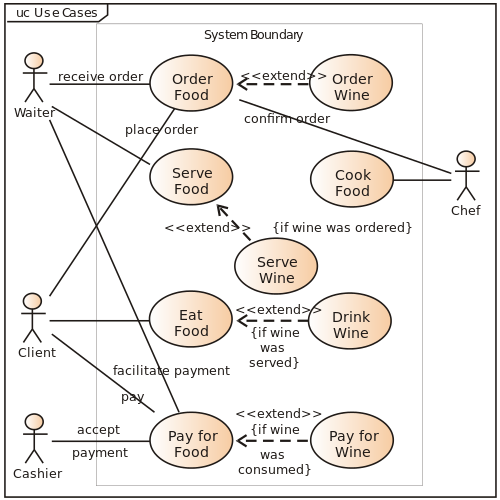
\includegraphics[width=0.35\textwidth]{use_case_restaurant_model}
  \caption{\label{fig:usecase} Un diagrama UML de casos de uso. Fuente: Wikimedia. Autor: Kishorekumar 62.}
\end{figure}

\subsection*{Subtítulo de ejemplo (colocar el nombre del módulo o componente en caso de una Descripción Técnica)}

\subsection*{Subtítulo de ejemplo (colocar la actividad como un sustantivo en caso de una Metodología)}

\section*{Especificación Técnica}%añadir pies de página

En esta sección se debe indicar claramente hasta dónde se va a llegar en el desarrollo del proyecto, es decir, delimitar la funcionalidad del proyecto. Para esto hay que realizar lo siguiente.

Indicar los lenguajes de programación a utilizar, los estándares, protocolos, manejadores de bases de datos, entornos de desarrollo, interfaces, componentes, etc., que se usarán en el desarrollo del proyecto. Por ejemplo, si se hará uso de un servicio remoto o si se hará una conexión a un dispositivo externo se deberá especificar el protocolo de comunicación usado. No se deberán describir las características de éstos elementos.

Especificar la magnitud de los datos que se manejarán, por ejemplo, si se propone un sistema de información se deberá indicar la cantidad de registros y usuarios simultáneos que debe ser capaz de soportar, mientras que si se propone un algoritmo se deberá indicar el tamaño de la instancia máxima que debe poder resolver y en cuánto tiempo.

Adicionalmente, se definirán las características mínimas que tendrá el producto final para dar por concluido el proyecto, esto se puede lograr explicando cómo se considerará que cada módulo a desarrollar o etapa de la metodología ya ha sido finalizado.

Para que la propuesta pueda ser aceptada, el último párrafo de esta sección deberá decir exactamente lo siguiente:

Al concluir el proyecto de integración se entregará un disco compacto al Coordinador de Estudios de Ingeniería en Computación que incluirá el reporte final del proyecto en un archivo PDF (sin restricciones)\footnote{Debe poder visualizarse sin solicitar contraseña}, el código fuente de la aplicación en un archivo comprimido (sin restricciones)\footnote{Debe poder descomprimirse sin solicitar contraseña}. La sección de apéndices del reporte final contendrá al menos un listado del código fuente desarrollado.

Adicionalmente a éste párrafo, el alumno especificará si se entregarán otros elementos como manuales de usuario, manuales de instalación, diagramas u otros elementos generados durante el desarrollo del proyecto. El disco compacto que se entregue al Coordinador de Estudios no deberá incluir ningún archivo ejecutable o multimedia, ni tampoco documentos o programas no desarrollados por los alumnos.

\section*{Cronograma de Actividades}

Se creará una tabla por cada una de las UEA que se contempla cursar durante la realización del proyecto, para cada una se incluirá el trimestre en el que se cursará, el nombre, la clave, el número de créditos y la cantidad de horas a cubrir (multiplicando 11 por el número de créditos).

Cada tabla de actividades estará referenciada en el texto y se le colocará una nota al pie de tabla con una descripción breve de su contenido. Hay que considerar que la suma de las horas invertidas en cada actividad tiene que coincidir con las horas esperadas de trabajo dependiendo la UEA a cursar. Un ejemplo de lo que se espera en esta tabla es:

El cronograma de actividades a realizar en el trimestre 2018 Invierno como parte de la UEA Proyecto de Integración de Ingeniería en Computación I con clave 1100113 de 18 créditos con un total de 198 horas se muestra en la Tabla~\ref{table:calendar}.

\begin{table}[h!]
  \begin{tabular}{p{0.3\textwidth} p{0.3\textwidth} p{0.3\textwidth}}
    \toprule
    \textbf{{Actividad}} & \textbf{{Horas}} & \textbf{{Producto}} \\
    \toprule
    Nombre de la actividad (comenzará con un verbo en infinitivo) &
    100 &
    Producto que se obtiene al finalizar la actividad (diagramas, documentación, código fuente, archivo de ejecución por lotes, etc.)\\
    \midrule
    Nombre de la actividad &
    98 &
    Producto que se obtiene al finalizar la actividad\\
    \midrule
    \textbf{Total} & 198 horas & \\
    \bottomrule
  \end{tabular}
  \caption{Calendario de actividades para el trimestre 2018 Invierno.}
  \label{table:calendar}
\end{table}

%Integrar esta sección dentro de factibilidad
\section*{Factibilidad}

En esta sección el autor explicará por qué su propuesta es realizable. Para esto, el autor evaluará la factibilidad desde el punto de vista operativo, técnico y económico.

La factibilidad operativa consiste en evaluar si todas las actividades planteadas en el calendario son realizables. Teniendo en cuenta un proyecto científico, una actividad no realizable sería tratar de romper una clave SHA-256 dado que ese problema es NP. Otra actividad de la misma índole sería la ejecución de una heurística que tarda 190 horas considerando un proyecto de 198 horas; el problema radicaría en que, si bien, no se sobrepasa el tiempo límite del proyecto, no se estaría considerando que los resultados pueden ser diferentes a los esperados, lo que quizás implique otra ronda de ejecución de experimentos.

La factibilidad técnica es el resultado de evaluar si los recursos humanos poseen los conocimientos y habilidades para llevar a cabo las actividades que se plantean en el calendario, por ejemplo, si el autor menciona que va a emplear \textit{Python} para implementar uno de los módulos que presentó en la Descripción Técnica, entonces, en este apartado debe indicar que conoce el lenguaje de programación en cuestión. La factibilidad técnica también incluye una lista y descripción de los recursos que no sean de uso común, por ejemplo, un servidor, un celular, una tarjeta de desarrollo, etc. Si se utiliza algún software que requiera licencia para utilizarlo, deberá indicarse que ya se tiene disponible al igual que los permisos para utilizarlo, si se utilizará alguna información especial, también se debe indicar si se tiene disponible y que se tiene el permiso para utilizarla. 

Por último, la factibilidad económica trata sobre una evaluación de los costos que implica la realización del proyecto en términos de uso de infraestructura, por ejemplo, computadoras, servidores, teléfonos inteligentes, conmutadores, encaminadores; todo el equipo físico en general. Además, se deben incluir gastos como acceso a Internet, uso de licencias, consumo de energía eléctrica y, en su caso, transporte, alimento y otros insumos. Asimismo, se deberá incluir el valor del trabajo intelectual, es decir, el costo por el tiempo invertido en el diseño y la implementación del proyecto. Esto daría una idea del capital mínimo que tendría el proyecto en caso de que se quisiera comercializar.

Para que la propuesta pueda ser aceptada, esta sección deberá contar con el siguiente párrafo (adaptado a número y género de los asesores). 

El asesor se responsabiliza de guiar al alumno y de que todos los recursos mencionados en la factibilidad técnica estarán disponibles para el alumno, de modo que el proyecto de integración se pueda concluir en tiempo y forma.\\[1.5cm]

%Cerrar esta sección con una conclusión
\begin{center}
  \begin{minipage}{0.4\textwidth}
    \centering
    Dra. Asesora %grado y nombre completo del asesor
  \end{minipage}
  \begin{minipage}{0.4\textwidth}
    \centering
    Dra. Coasesora %grado y Nombre completo del coasesor
  \end{minipage}
\end{center}%Escribe tu propuesta en este archivo
    
    %Este archivo define el estilo IEEE de las referencias en español
    \small
    \bibliographystyle{IEEEtran}
    \bibliography{piic}%Añade las referencias que necesites en el archivo .bib
    
\end{document}